\section{The Formal Semantics of ForeC}
\label{sec:formalSemantics}
This section presents the formal semantics of ForeC as rewrite rules,
in the style of Structural Operation Semantics~\cite{semantics_sos}. The rewrite rules 
define the possible transitions between program states. We define the
semantics on a set of primitive (kernel) ForeC statements, from which 
the full set of ForeC statements is derived from. This simplifies the 
formal definition of the ForeC language. The kernel statements are 
given in Figure~\ref{fig:forec_kernel} and only considers a subset of 
the C language because we are focusing on the ForeC semantics.
This section continues by defining how the program variables, in particular 
shared variables, are represented in the semantics. Then, the 
notation of the rewrite rules is given, followed by the ForeC semantics.

\begin{figure}[!h]
	\centering

%	\renewcommand{\arraystretch}{1.25}
	\begin{tabular}{l l l}
		\verb$nop$																& & Empty statement					\\
		\verb$pause$															& & Barrier synchronisation			\\
		\emph{tq v}																& & Variable declaration			\\
		\emph{v = exp}															& & Assignment						\\
		\emph{t}\verb$;$~\emph{u}												& & Sequence						\\
		\verb$if$~(\emph{exp})~\emph{t}~\verb$else$~\emph{u}					& & Conditional						\\
		\verb$while$~(\emph{exp})~\emph{t}										& & Loop							\\
		\verb$par($\emph{t},~\emph{u}\verb$)$									& & Fork/join parallelism			\\
		\verb$weak$?~\verb$abort$~\emph{t}~\verb$when imm$?~\emph{exp}			& & Structured preemption
	\end{tabular}
	
	\caption{The ForeC kernel statements. Here, \emph{tq} is a type-qualifier, \emph{v} is a variable, 
			 \emph{exp} is an expression, \emph{t} and \emph{u} are arbitrary kernel statements, and 
			 \emph{imm} is short for \emph{immediate}.}
	\label{fig:forec_kernel}
\end{figure}

%-----------------------------------------------------------------------------

\subsection{The Program Environment}
The layout and contents of the program memory is described by 
the program environment \emph{E}, which is a function that maps 
variables (\emph{Var}) to values (\emph{Val}) and type-qualifier 
information (\emph{Type1} and \emph{Type2}):
\begin{equation*}
	E: Var \to \langle Val,~Type1,~Type2 \rangle
\end{equation*}
\emph{Type1} is \emph{pvt} or \emph{shd} if the variable is 
private or shared, respectively. \emph{Type2} is \emph{out} 
or \emph{ord} if the variable is or is not an output variable, 
respectively. A variable declaration updates \emph{E} with a
new mapping. For example, the declaration ``\verb$int x=1$'' 
updates \emph{E} with a mapping from \verb$x$ to $\langle 1,~pvt,~ord \rangle$. 
Input variables are mapped to values in a separate 
environment \emph{I}. 

To handle variable scoping, a new \emph{local} environment 
is made when execution enters a new scope. Variables declared 
in the new scope will update the new local environment. Each 
scope is given a unique identifier and a variable declaration 
(\emph{var}) in a given scope (\emph{scope}) is referred to as 
$var_{scope}$. The program environment \emph{E} is initially 
defined by the global environment $E_\mathcal{G}$ containing the 
global variables. When a new scope is entered, 
its local environment is appended to \emph{E}. When the scope 
ends, its local environment is removed from \emph{E}. 
Threads are always implicitly scoped and a \verb$par$ appends the 
local environments of the child threads to the parent's local 
environment, creating a tree-like structure. To find a variable 
declaration, the search starts from the current scope of execution 
and proceeds up the tree until it is found. For example, in
\begin{lstlisting}[style=snippet]
// Scope (*$\mathcal{G}$*)
int x=0;
void main(void) { // Scope 0
  int v = 1;
  par( {/*Scope 1*/ int x; x=2; (*$\bullet$*)} , {/*Scope 2*/ x=3; (*$\bullet$*)} );
  int w = 4;
}
\end{lstlisting}
the program environment just before both threads terminate 
(indicated by the $\bullet$) is shown in Figure~\ref{fig:shared_before_term},
where $E_\mathcal{G}$ is the root of the tree and the scope of each 
\emph{E} is given by its subscript. In the program, the first 
thread made its assignment to the declaration of \verb$x$ in $E_1$, 
while the second thread made its assignment to the declaration 
of \verb$x$ in $E_\mathcal{G}$.

\begin{figure}[t]
	\centering
	
	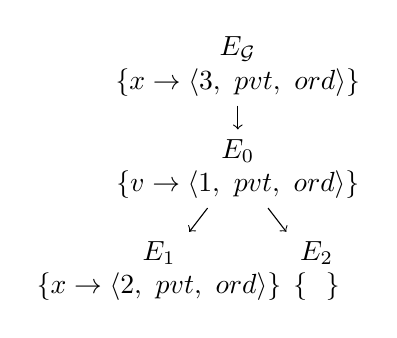
\begin{tikzpicture}[->]
		\node[align=center] (E_G) at (0, 0) {$E_\mathcal{G}$\\$\{x \to \langle 3,~pvt,~ord \rangle\}$};
		\node[align=center] (E_0) at (0, -1.3) {$E_0$\\$\{v \to \langle 1,~pvt,~ord \rangle\}$};
		\node[align=center] (E_1) at (-1, -2.6) {$E_1$\\$\{x \to \langle 2,~pvt,~ord \rangle\}$};
		\node[align=center] (E_2) at (1, -2.6) {$E_2$\\$\{~~\}$};
		\draw (E_G) -- (E_0);
		\draw (E_0) -- (E_1);
		\draw (E_0) -- (E_2);
	\end{tikzpicture}
	
	\caption{The program environment just before both threads terminate.}
	\label{fig:shared_before_term}
\end{figure}


%-----------------------------------------------------------------------------

\subsection{The Thread Environment}
Threads maintain their copies of shared variables in their own 
thread environment \emph{S}, which is a function that maps copies 
of shared variables (\emph{Var}) to values (\emph{Val}) and modify 
statuses (\emph{Mod}):
\begin{equation*}
	S: Var \to \langle Val,~Mod \rangle
\end{equation*}
\emph{Mod} is used to track which copies have been assigned a new 
value or have been copied by other threads. The value of \emph{Mod} 
is either \emph{true}, \emph{false}, or \emph{copied}.
The default value of \emph{Mod} for a copy is \emph{false}, 
but it is set to \emph{true} whenever the copy is assigned 
a new value. If the copy is copied by another thread, then \emph{Mod} 
is set to \emph{copied}. Like the program environment \emph{E}, the 
thread environment \emph{S} maintains local environments to handle 
variable scoping. As a thread cannot access the variables of its 
siblings, \emph{S} does not branch and is, therefore, linear. For 
convenience, \emph{SS} is a function that maps threads (\emph{Thr}) 
to their thread environment:
\begin{equation*}
	SS: Thr \to \{S\}
\end{equation*}

A thread will only create copies of the shared variables that it may 
access. However, information about the shared variables that a thread 
may access is needed before execution. To this end, we traverse each 
thread and build the set of shared variables ($Var_{Scope}$) that it 
may access. A shared variable declaration, including its initialisation, 
is not treated as an access. $\mathcal{A}$ is a function that maps threads 
(\emph{Thr}) to the shared variables that they may access:
\begin{equation*}
	\mathcal{A}: Thr \to \{Var_{Scope}\}
\end{equation*}

\begin{algorithm}[t]
	\caption{$\mathcal{D}(E, SS, Thr)$ for creating thread environments.}
	\label{algo:aux_D}

	\begin{algorithmic}[1]
		\Require \emph{E}, \emph{SS}, and \emph{Thr} 
				 (program environment, existing thread environments, and set of child threads).
		\Ensure $\langle SS,~NewS \rangle$ (potentially modified input \emph{SS}, and new thread environments).

		\State $NewS: Thr \to \{S\}$
		\ForAll{$thr \in Thr$}	\label{algo:aux_D_each_thread1}
			\ForAll{$var_{scope} \in \mathcal{A}[thr]$} \label{algo:aux_D_each_var1}
				\State $found \gets false$
				\ForAll{$S_p \in \mathcal{P}(SS,~thr)$}	\label{algo:aux_D_each_p1}
					\If{$var_{scope} \in S_p$}
						\State $NewS[thr][var_{scope} \gets S_p[var_{scope}]]$	\label{algo:aux_D_found1}
						\State $S_p[var_{scope}].mod \gets copied$	\label{algo:aux_D_found2}
						\State $found \gets true$
						\State \textbf{break}
					\EndIf
				\EndFor	\label{algo:aux_D_each_p2}
				\If{$\lnot found \land var_{scope} \in E$}
					\State $NewS[thr][var_{scope} \gets \langle E[var_{scope}].val,~false \rangle ]$	\label{algo:aux_D_from_E}
				\EndIf
			\EndFor	\label{algo:aux_D_each_var2}
		\EndFor	\label{algo:aux_D_each_thread2}
		\State \Return $\langle SS,~NewS \rangle$
	\end{algorithmic}
\end{algorithm}

When a \verb$par$ executes, we use the auxiliary function $\mathcal{D}$ 
to create a new thread environment for each child thread. The thread 
environments are populated with the necessary copies of shared variables. 
The function is described by Algorithm~\ref{algo:aux_D}. The algorithm 
begins by defining \emph{NewS}, which maps the child threads to their 
new thread environment. 
For each child thread (Line~\ref{algo:aux_D_each_thread1}), 
the shared variables that it may access are copied into its thread environment
(Lines~\ref{algo:aux_D_each_var1} - \ref{algo:aux_D_each_var2}). 
If a copy of the shared variable is already in a predecessor's environment 
($S_p$), then that copy is copied (Lines~\ref{algo:aux_D_each_p1} - 
\ref{algo:aux_D_each_p2}). The function $\mathcal{P}(SS,~thr)$ returns the 
environments of thread \emph{thr}'s predecessors, starting from the 
parent through to its most distant predecessor. Lines~\ref{algo:aux_D_found1} and 
\ref{algo:aux_D_found2} updates the child thread's environment ($NewS[thr]$) 
with the predecessor's copy, which is subsequently marked as \emph{copied}. 
We use the infix `.' operator to access the elements in a tuple.
However, if a copy is not found, then a fresh 
copy is made from the program environment \emph{E} if available (Line~\ref{algo:aux_D_from_E}). 
A shared variable would not available if 
execution is outside of its declaration scope. For example, in
\begin{lstlisting}[style=snippet]
// Scope (*$\mathcal{G}$*)
int plus(int a, int b) {return a + b;}
shared int x=0 combine with plus;
void main(void) { // Thread main, Scope 0
  x=1;
  shared int y=0 combine with cf;
  par( {/*Thread 1, Scope 1*/ x=x+2;}, 
       {/*Thread 2, Scope 2*/ y=x;  } );
}
\end{lstlisting}
the shared variables that may be accessed by thread \verb$main$ are 
$\{x_\mathcal{G}\}$, by thread $1$ are $\{x_\mathcal{G}\}$, and by 
thread $2$ are $\{x_\mathcal{G},~y_0\}$. Figures~\ref{fig:shared_before_par}
and \ref{fig:shared_at_par} show the program and thread environments
just before the \verb$par$ executes and just before both child threads terminate, 
respectively. 

\begin{figure}[t]
	\centering
	\subfloat[Program] {
		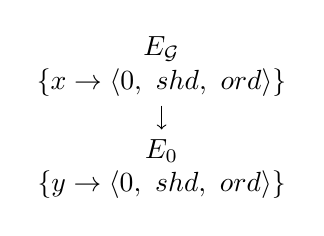
\begin{tikzpicture}[->]
			\node[align=center] (E_G) at (0, 0) {$E_\mathcal{G}$\\$\{x \to \langle 0,~shd,~ord \rangle\}$};
			\node[align=center] (E_0) at (0, -1.3) {$E_0$\\$\{y \to \langle 0,~shd,~ord \rangle\}$};
			\draw (E_G) -- (E_0);
		\end{tikzpicture}
	}
	\hspace{1cm}
	\subfloat[Thread main] {
		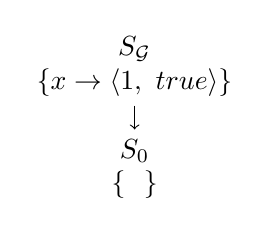
\begin{tikzpicture}[->]
			\node[align=center] (S_G) at (0, 0) {$S_\mathcal{G}$\\$\{x \to \langle 1,~true \rangle\}$};
			\node[align=center] (S_0) at (0, -1.3) {$S_0$\\$\{~~\}$};
			\draw (S_G) -- (S_0);
		\end{tikzpicture}
	}
	
	\caption{Environments just before the par.}
	\label{fig:shared_before_par}
\end{figure}

\begin{figure}[t]
	\centering
	\subfloat[Program] {
		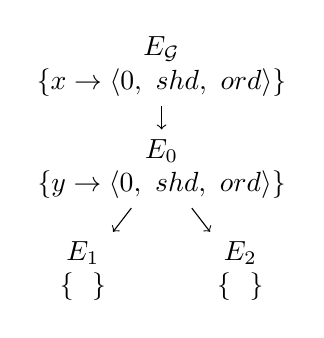
\begin{tikzpicture}[->]
			\node[align=center] (E_G) at (0, 0) {$E_\mathcal{G}$\\$\{x \to \langle 0,~shd,~ord \rangle\}$};
			\node[align=center] (E_0) at (0, -1.3) {$E_0$\\$\{y \to \langle 0,~shd,~ord \rangle\}$};
			\node[align=center] (E_1) at (-1, -2.6) {$E_1$\\$\{~~\}$};
			\node[align=center] (E_2) at (1, -2.6) {$E_2$\\$\{~~\}$};
			\draw (E_G) -- (E_0);
			\draw (E_0) -- (E_1);
			\draw (E_0) -- (E_2);
		\end{tikzpicture}
	}
	\hfill
	\subfloat[Thread main] {
		\begin{tikzpicture}[->]
			\node[align=center] (S_G) at (0, 0) {$S_\mathcal{G}$\\$\{x \to \langle 1,~copied \rangle\}$};
			\node[align=center] (S_0) at (0, -1.3) {$S_0$\\$\{~~\}$};
			\node                     at (0, -2.975) {~~~~~~~~~~~~~~~~~~~};
			\draw (S_G) -- (S_0);
		\end{tikzpicture}
	}
	\hfill
	\subfloat[Thread 1] {
		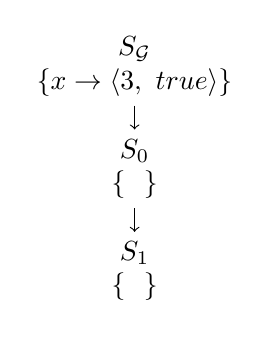
\begin{tikzpicture}[->]
			\node[align=center] (S_G) at (0, 0) {$S_\mathcal{G}$\\$\{x \to \langle 3,~true \rangle\}$};
			\node[align=center] (S_0) at (0, -1.3) {$S_0$\\$\{~~\}$};
			\node[align=center] (S_1) at (0, -2.6) {$S_1$\\$\{~~\}$};
			\draw (S_G) -- (S_0);
			\draw (S_0) -- (S_1);
		\end{tikzpicture}
	}
	\hfill
	\subfloat[Thread 2] {
		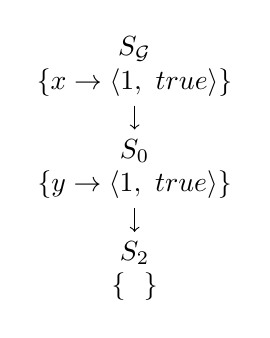
\begin{tikzpicture}[->]
			\node[align=center] (S_G) at (0, 0) {$S_\mathcal{G}$\\$\{x \to \langle 1,~true \rangle\}$};
			\node[align=center] (S_0) at (0, -1.3) {$S_0$\\$\{y \to \langle 1,~true \rangle\}$};
			\node[align=center] (S_2) at (0, -2.6) {$S_2$\\$\{~~\}$};
			\draw (S_G) -- (S_0);
			\draw (S_0) -- (S_2);
		\end{tikzpicture}
	}

	\caption{Environments just before the child threads terminate.}
	\label{fig:shared_at_par}
\end{figure}

For the kernel semantics, we assume that the combine function 
is specified with the \verb$shared$ type-qualifier, such as 
``\verb$shared:$\emph{cf}'' where \emph{cf} is the combine function. 
$\mathcal{C}$ is a function that maps shared variables ($Var_{Scope}$) 
to their combine function:
\begin{equation*}
	\mathcal{C}: Var_{Scope} \to \{cf\}
\end{equation*}

When a global tick ends or when a \verb$par$ terminates, we use 
the auxiliary function $\mathcal{C}omb$ to combine the modified 
copies of each shared variable in a given set of thread environments. 
The combined values are then assigned to a specified environment. 
The function is described by Algorithm~\ref{algo:aux_C}. 
For each shared variable (Line~\ref{algo:aux_C_each_var}), the algorithm 
builds a set of copies from the given thread environments. 
From this, a new set is built, containing only the values of 
the modified copies. If there is at least one value in \emph{Values}, 
Line~\ref{algo:aux_C_result1} removes a value and assigns it to \emph{result}. 
Line~\ref{algo:aux_C_result2} combines the remaining values with 
\emph{result}, using the shared variable's combine function \emph{cf}. 
Finally, Line~\ref{algo:aux_C_result3} assigns the combined value to 
the shared variable in the given environment \emph{A}. If \emph{A}
is a thread environment, then the variable's modify status (\emph{Mod})
is automatically set to \emph{true}. For the previous example
program, Figure~\ref{fig:shared_after_par} gives the program and thread 
environments after the \verb$par$ has terminated.

\begin{algorithm}[t]
	\caption{$\mathcal{C}omb(\{S\}, A)$ for combining copies of shared variables in a set of thread environments.}
	\label{algo:aux_C}

	\begin{algorithmic}[1]
		\Require $\{S\}$ and \emph{A} (set of thread environments, and environment to assign the combined values).
		\Ensure \emph{A} (Modified input \emph{A}).

		\ForAll{shared $var_{scope}$ in the program environment}	\label{algo:aux_C_each_var}
			\State $Copies \gets \{S[var_{scope}]~|~var_{scope} \in S)\}$
			\State $Values \gets \{copy.val~|~copy.mod = true,~copy \in Copies\}$
			\If{$Values$ is not empty}
				\State $result \gets value \in Values,~Values \gets Values \setminus \{value\}$ \label{algo:aux_C_result1}
				\ForAll{$value \in Values$}
					\State $result \gets cf(value,~result),~cf = \mathcal{C}[var_{scope}]$ \label{algo:aux_C_result2}
				\EndFor
				\State $A[var_{scope}].val \gets result$ \label{algo:aux_C_result3}
			\EndIf
		\EndFor
		\State \Return \emph{A}
	\end{algorithmic}
\end{algorithm}

\begin{figure}[t]
	\centering
	\subfloat[Program] {
		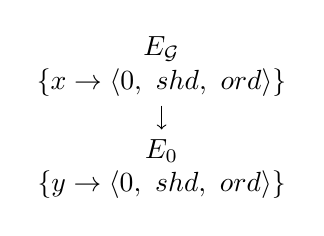
\begin{tikzpicture}[->]
			\node[align=center] (E_G) at (0, 0) {$E_\mathcal{G}$\\$\{x \to \langle 0,~shd,~ord \rangle\}$};
			\node[align=center] (E_0) at (0, -1.3) {$E_0$\\$\{y \to \langle 0,~shd,~ord \rangle\}$};
			\draw (E_G) -- (E_0);
		\end{tikzpicture}
	}
	\hspace{1cm}
	\subfloat[Thread main] {
		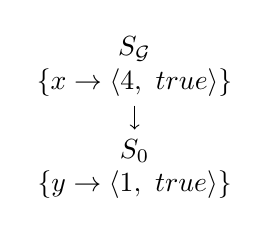
\begin{tikzpicture}[->]
			\node[align=center] (S_G) at (0, 0) {$S_\mathcal{G}$\\$\{x \to \langle 4,~true \rangle\}$};
			\node[align=center] (S_0) at (0, -1.3) {$S_0$\\$\{y \to \langle 1,~true \rangle\}$};
			\draw (S_G) -- (S_0);
		\end{tikzpicture}
	}
	
	\caption{Environments after the par.}
	\label{fig:shared_after_par}
\end{figure}

When an expression is evaluated, the values of private and shared 
variables are taken from the program's environment \emph{E} and 
the enclosing thread environment \emph{S}, respectively. Expressions
may have \emph{side-effects}, where variables in \emph{E} and \emph{S} 
may be assigned new values. To evaluate an expression, we use an auxiliary 
function $\mathcal{E}$ which maps the environment of the program and 
enclosing thread, the inputs, and the expression to the value of the 
expression and possibly updated environments. The signature of $\mathcal{E}$ is:
\begin{equation*}
		\mathcal{E}: E \times S \times I \times exp \to \langle val,~E',~S' \rangle
\end{equation*}


%-----------------------------------------------------------------------------

\subsection{Inlining of Functions}
The execution of a function call requires the instantiation and 
initialisation of its parameters before the function body can 
execute. This initialisation phase complicates the design of the
semantic rules. For simplicity, the semantic rules do not consider 
function calls and we assume all functions have been inlined at 
their call site.

%-----------------------------------------------------------------------------

\subsection{Notation}
The rewrite rules, in the style of Structural Operational Semantics, 
have the following form:
\begin{equation*}
	E, SS: t \xrightarrow[~~I~~]{k} E', SS': t'
\end{equation*}
where,
\begin{itemize}
	\item $E$ and $E'$ is the program environment before and after the transition, respectively.
	\item $SS$ and $SS'$ is the thread environments before and after the transition, respectively.
	\item $I$ maps the input variables to values. 
	\item $t$ and $t'$ is an arbitrary composition of kernel statements before and after the transition, respectively.
	\item $k$ is the completion code of the transition.
\end{itemize}

This notation describes a program fragment \emph{t}, called a \emph{term}, transitioning from 
the state $E, SS: t$ to $E', SS': t'$ with the inputs \emph{I}. A state is defined 
by \emph{t} and the environments \emph{E} and \emph{SS}. Each transition finishes 
with a completion code of \emph{k}, encoding the execution status of the transition:

\begin{itemize}
	\item If \emph{k = 0}, then the execution of \emph{t} terminates.
	\item If \emph{k = 1}, then the execution of \emph{t} pauses for the current global tick, but 
		  resumes at the next global tick.
	\item If \emph{k = $\bot$}, then the execution of \emph{t} continues for the current global tick.
\end{itemize}

Transitions may depend on how some sub-terms are rewritten or on some values in \emph{E}
and \emph{SS}. This dependency is expressed with deduction rules of the following form:
\begin{equation*}
	\frac{
			\dotsm
		}{
			E, SS: t \xrightarrow[~~I~~]{k} E', SS': t'
		}
\end{equation*}
where the premise (`$\dotsm$' above the bar) must hold for the conclusion (below the bar) 
to proceed.

To denote a sequence of transitions, where all but the last transition has 
a completion code of $\bot$, the ``$\xRightarrow{~~~~~}$'' arrow is used 
instead. For example, the transition
\begin{equation*}
	E, SS: t \xRightarrow[~~I~~]{k} E', SS': t'
\end{equation*}
corresponds to the following sequence of transitions:
\begin{equation*}
	E, SS: t \xrightarrow[~~I~~]{\bot} E_1, SS_1: t_1 \xrightarrow[~~I~~]{\bot} \cdots E_n, SS_n: t_n \xrightarrow[~~I~~]{k} E', SS': t'
\end{equation*}
where \emph{k} is $0$ or $1$.

%-----------------------------------------------------------------------------

\subsection{The Structural Operational Semantics}

\noindent (nop) The empty statement does nothing and terminates instantly, 
leaving no residue:
\begin{equation*}	
	\tag{nop}
	\label{forec:nop}
	E, SS: nop 
		\xrightarrow[~~I~~]{0} 
	E, SS: 
\end{equation*}

\noindent (pause) The \verb$pause$ statement pauses for the current global 
tick and rewrites into \emph{nop}:
\begin{equation*}
	\tag{pause}
	\label{forec:pause}
	E, SS: pause 
		\xrightarrow[~~I~~]{1} 
	E, SS: nop
\end{equation*}

\noindent (declare) The following declaration rules do not apply to global 
variables because the program environment \emph{E} is initially
populated with the global declarations. As input and output variables 
can only be global variables, the following rules also do not apply 
to them. A variable declaration updates the program's environment \emph{E}
with the variable and associated tuple $\langle 0,~type1,~type2 \rangle$.
The tuple is created from the variable's type qualifier by the auxiliary 
function $\mathcal{T}(tq)$. A private variable declaration does not have
\verb$shared$ in its type-qualifier:
\begin{equation*}
	\tag{declare1}
	\label{forec:declare1}
	\frac{
			shared \notin tq
			\quad
			E' = E[v \gets \mathcal{T}(tq)]
		}{
			E, SS: tq~v 
				\xrightarrow[~~I~~]{0} 
			E', SS: 
		}
\end{equation*}
For a shared variable, the combine function is also recorded:
\begin{equation*}
	\tag{declare2}
	\label{forec:declare2}
	\frac{
			shared \in tq
			\quad
			v \notin A[thr]
			\qquad
			\mathcal{C}[v \gets cf \in tq]
			\quad
			E' = E[v \gets \mathcal{T}(tq)]
		}{
			E, SS: tq~v 
				\xrightarrow[~~I~~]{0} 
			E', SS: 
		}
\end{equation*}
If the shared variable is declared in a thread that may access it, 
a copy is also made for the thread:
\begin{equation*}
	\tag{declare3}
	\label{forec:declare3}
	\frac{
		\twolines{
				shared \in tq
				\quad
				v \in A[thr]
			}{
				\mathcal{C}[v \gets cf \in tq]
				\quad
				E' = E[v \gets \mathcal{T}(tq)]
				\quad
				SS' = SS[thr][v \gets \langle 0, false \rangle]
			}
		}{
			E, SS: tq~v 
				\xrightarrow[~~I~~]{0} 
			E', SS': 
		}
\end{equation*}

\noindent (assign) An assignment to a private variable updates the 
variable in \emph{E} with the value of the expression. An assignment 
to a shared variable updates the thread's copy of the variable with 
the value of the expression. Side-effects in the expression may update 
\emph{E} and \emph{SS} as well. Assignments to input 
variables, being read-only, are syntactically forbidden:
\begin{equation*}
	\tag{assign1}
	\label{forec:assign1}
	\frac{
		\twolines{
				E[v].type1 \neq shd
			}{
				\langle val, E', SS'[thr] \rangle = \mathcal{E}(E, SS[thr], I, exp)
				\qquad
				E'' = E'[v].val \gets val
			}
		}{
			E, SS: v = exp 
				\xrightarrow[~~I~~]{0} 
			E'', SS': 
		}
\end{equation*}

\begin{equation*}
	\tag{assign2}
	\label{forec:assign2}
	\frac{
		\twolines{
				E[v].type1 = shd
			}{
				\langle val, E', SS'[thr] \rangle = \mathcal{E}(E, SS[thr], I, exp)
				\qquad
				SS'' = SS'[thr][v].val \gets val
			}
		}{
			E, SS: v = exp 
				\xrightarrow[~~I~~]{0} 
			E', SS'': 
		}
\end{equation*}

\noindent(seq) If the first term pauses, then the sequence 
behaves as a \verb$pause$. Otherwise, the sequence is rewritten into its 
second term:
\begin{equation*}
	\tag{seq1}
	\label{forec:seq1}
	\frac{
			E, SS: t 
				\xRightarrow[~~I~~]{1} 
			E', SS': t'
		}{
			E, SS: t;u 
				\xrightarrow[~~I~~]{1} 
			E', SS': t';u
		}
\end{equation*}

\begin{equation*}
	\tag{seq2}
	\label{forec:seq2}
	\frac{
			E, SS: t
				\xRightarrow[~~I~~]{0} 
			E', SS': 
		}{
			E, SS: t;u 
				\xrightarrow[~~I~~]{\bot} 
			E', SS': u
		}
\end{equation*}

\noindent (cond) The \verb$if$-statement is rewritten into one of 
its branches, depending on the expression:
\begin{equation*}
	\tag{cond1}
	\label{forec:cond1}
	\frac{
			\langle val, E', SS'[thr] \rangle = \mathcal{E}(E, SS[thr], I, exp)
			\qquad
			val \neq 0
		}{
			E, SS: if~(exp)~t~else~u
				\xrightarrow[~~I~~]{\bot} 
			E', SS': t
		}
\end{equation*}

\begin{equation*}
	\tag{cond2}
	\label{forec:cond2}
	\frac{
			\langle val, E', SS'[thr] \rangle = \mathcal{E}(E, SS[thr], I, exp)
			\qquad
			val = 0 
		}{
			E, SS: if~(exp)~t~else~u
				\xrightarrow[~~I~~]{\bot} 
			E', SS': u
		}
\end{equation*}

\noindent (loop) The body of the \verb$while$-statement is unrolled 
once if the expression does not evaluate to a zero value. Otherwise, 
the statement is terminated:
\begin{equation*}
	\tag{loop1}
	\label{forec:loop1}
	\frac{
			\langle val, E', SS'[thr] \rangle = \mathcal{E}(E, SS[thr], I, exp)
			\qquad
			val \neq 0
		}{
			E, SS: while~(exp)~t
				\xrightarrow[~~I~~]{\bot} 
			E', SS': t; while~(exp)~t
		}
\end{equation*}

\begin{equation*}
	\tag{loop2}
	\label{forec:loop2}
	\frac{
			\langle val, E', SS'[thr] \rangle = \mathcal{E}(E, SS[thr], I, exp)
			\qquad
			val = 0
		}{
			E, SS: while~(exp)~t
				\xrightarrow[~~I~~]{0} 
			E', SS': 
		}
\end{equation*}

\noindent (par) The \verb$par$ statement allows both terms (threads) to 
execute. In the premise, the auxiliary function $\mathcal{D}$ creates 
new thread environments ($S_t$ and $S_u$) for each term. The terms execute
with their new thread environment until they pause or terminate. If both 
terms pause, then the \verb$par$ 
behaves as a \verb$pause$. If only one term terminates, then the \verb$par$ 
is rewritten into its remaining term. As only private variables can be 
updated in \emph{E}, the updates in $E'$ and $E''$ are mutually exclusive. 
Hence, the resulting program environment is composed of updates from 
$E'$ and $E''$, denoted $E' \oplus E''$. The execution of a term can only
update $SS'$ with new thread environments from nested threads or set the \emph{Mod} 
value of some copies to \emph{copied}. Thus, the resulting thread environments
is composed of $S_t'$, $S_u'$, and the merging of $SS''$ and $SS'''$ such that 
the new \emph{Mod} values are kept. This is denoted $(SS'' \oplus SS''')[t \gets S_t', u \gets S_u']$:
\begin{equation*}
	\tag{par1}
	\label{forec:par1}
	\frac{
		\twolines{
				\langle SS', \{S_t, S_u\} \rangle = \mathcal{D}(E, SS, \{t, u\})
			}{
				E, SS'[t \gets S_t]: t
					\xRightarrow[~~I~~]{1} 
				E', SS''[t \gets S_t']: t'
				\qquad
				E, SS'[u \gets S_u]: u
					\xRightarrow[~~I~~]{1} 
				E'', SS'''[u \gets S_u']: u'
			}
		}{
			E, SS: par(t,u) 
				\xrightarrow[~~I~~]{1} 
			E' \oplus E'', (SS'' \oplus SS''')[t \gets S_t', u \gets S_u']: par(t',u')
		}
\end{equation*}

\begin{equation*}
	\tag{par2}
	\label{forec:par2}
	\frac{
		\twolines{
				\langle SS', \{S_t, S_u\} \rangle = \mathcal{D}(E, SS, \{t, u\})
			}{
				E, SS'[t \gets S_t]: t
					\xRightarrow[~~I~~]{1} 
				E', SS''[t \gets S_t']: t'
				\qquad
				E, SS'[u \gets S_u]: u
					\xRightarrow[~~I~~]{0} 
				E'', SS'''[u \gets S_u']:
			}
		}{
			E, SS: par(t,u) 
				\xrightarrow[~~I~~]{1} 
			E' \oplus E'', (SS'' \oplus SS''')[t \gets S_t', u \gets S_u']: t'
		}
\end{equation*}

\begin{equation*}
	\tag{par3}
	\label{forec:par3}
	\frac{
		\twolines{
				\langle SS', \{S_t, S_u\} \rangle = \mathcal{D}(E, SS, \{t, u\})
			}{
				E, SS'[t \gets S_t]: t
					\xRightarrow[~~I~~]{0} 
				E', SS''[t \gets S_t']: 
				\qquad
				E, SS'[u \gets S_u]: u
					\xRightarrow[~~I~~]{1} 
				E'', SS'''[u \gets S_u']: u'
			}
		}{
			E, SS: par(t,u) 
				\xrightarrow[~~I~~]{1} 
			E' \oplus E'', (SS'' \oplus SS''')[t \gets S_t', u \gets S_u']: u' 
		}
\end{equation*}
If both terms terminate, then the \verb$par$ terminates and the thread 
environments of both terms ($S_t$ and $S_u$) are combined and assigned 
to the parent thread's environment $S_p$, where \emph{p} denotes the 
parent thread:
\begin{equation*}
	\tag{par4}
	\label{forec:par4}
	\frac{
		\twolines{
				\langle SS', \{S_t, S_u\} \rangle = \mathcal{D}(E, SS, \{t, u\})
			}{
				\twolines{
					E, SS'[t \gets S_t]: t
						\xRightarrow[~~I~~]{0} 
					E', SS''[t \gets S_t']:
					\qquad
					E, SS'[u \gets S_u]: u
						\xRightarrow[~~I~~]{0} 
					E'', SS'''[u \gets S_u']:
				}{
					S_p' = \mathcal{C}omb(\{S_t', S_u'\}, S_p \in SS)
				}
			}
		}{
			E, SS: par(t,u) 
				\xrightarrow[~~I~~]{0} 
			E' \oplus E'', (SS'' \oplus SS''')[p \gets S_p']:
		}
\end{equation*}

\noindent (abort) 
The only difference between a delayed \verb$abort$ and an immediate \verb$abort$ is 
whether or not the expression is evaluated the first time the \verb$abort$ 
is executed. The expression is not evaluated for a delayed \verb$abort$, 
but it is evaluated for an immediate \verb$abort$. In subsequent 
global ticks, the execution behaviour of both variants is identical. 
Hence, a delayed abort is rewritten into its 
immediate variant:
\begin{equation*}
	\tag{abort1}
	\label{forec:abort1}
	\frac{
			E, SS: t
				\xRightarrow[~~I~~]{1} 
			E', SS': t'
		}{
			E, SS: weak?~abort~t~when~exp
				\xrightarrow[~~I~~]{1} 
			E', SS': weak?~abort~t'~when~imm~exp
		}
\end{equation*}
A delayed abort terminates if its body terminates:
\begin{equation*}
	\tag{abort2}
	\label{forec:abort2}
	\frac{
			E, SS: t
				\xRightarrow[~~I~~]{0} 
			E', SS':
		}{
			E, SS: weak?~abort~t~when~exp
				\xrightarrow[~~I~~]{0} 
			E', SS':
		}
\end{equation*}
An immediate abort allows its body to execute normally if preemption is 
not triggered (the expression evaluates to a zero value):
\begin{equation*}
	\tag{abort3}
	\label{forec:abort3}
	\frac{
			\langle val, E', SS'[thr] \rangle = \mathcal{E}(E, SS[thr], I, exp)
			\qquad
			val = 0
			\qquad
			E', SS': t
				\xRightarrow[~~I~~]{1} 
			E'', SS'': t'
		}{
			E, SS: weak?~abort~t~when~imm~exp
				\xrightarrow[~~I~~]{1} 
			E'', SS'': weak?~abort~t'~when~imm~exp
		}
\end{equation*}

\begin{equation*}
	\tag{abort4}
	\label{forec:abort4}
	\frac{
			\langle val, E', SS'[thr] \rangle = \mathcal{E}(E, SS[thr], I, exp)
			\qquad
			val = 0
			\qquad
			E', SS': t
				\xRightarrow[~~I~~]{0} 
			E'', SS'': 
		}{
			E, SS: weak?~abort~t~when~imm~exp
				\xrightarrow[~~I~~]{0} 
			E'', SS'': 
		}
\end{equation*}
A strong and immediate abort terminates when preemption is triggered
(the expression evaluates to a non-zero value). The body is not executed:
\begin{equation*}
	\tag{abort5}
	\label{forec:abort5}
	\frac{
			\langle val, E', SS'[thr] \rangle = \mathcal{E}(E, SS[thr], I, exp)
			\qquad
			val \neq 0
		}{
			E, SS: abort~t~when~imm~exp
				\xrightarrow[~~I~~]{0} 
			E', SS': 
		}
\end{equation*}
A weak and immediate abort allows its body to execute one last time 
when preemption is triggered:
\begin{equation*}
	\tag{abort6}
	\label{forec:abort6}
	\frac{
		\twolines{
				\langle val, E', SS'[thr] \rangle = \mathcal{E}(E, SS[thr], I, exp)
				\qquad
				val \neq 0
			}{
				E', SS': t
					\xRightarrow[~~I~~]{k} 
				E'', SS'': t'
				\qquad
				k \in \{0, 1\}
			}
		}{
			E, SS: weak~abort~t~when~imm~exp
				\xrightarrow[~~I~~]{0} 
			E'', SS'': 
		}
\end{equation*}

\noindent (prog) The following rule defines the program's execution for a
global tick. The term $t$ corresponds to the program at the start of the 
global tick and $t'$ is the residue of the program at the end of the global tick. 
At the program's initial global tick, $SS$ is empty.
Before the program executes, the input variables are updated using the 
auxiliary function $updateInputs(~)$, defined by the implementation.
Also, a new thread environment ($S_{main}$) is created for the program's 
\verb$main$ function.
After the program completes the global tick, by pausing or terminating, 
all the shared variables are combined. The output variables are emitted using the 
auxiliary function $emitOutputs(E)$, defined by the implementation:
\begin{equation*}
	\tag{prog}
	\label{forec:prog}
	\frac{
		\twolines{
				SS = \{~~\}
				\qquad
				I = updateInputs(~)
				\qquad
				\langle SS', \{S_{main}\} \rangle = \mathcal{D}(E, SS, \{main\})
			}{
				\twolines{
					E, SS'[main \gets S_{main}]: t
						\xRightarrow[~~I~~]{k} 
					E', SS''[main \gets S_{main}']: t'
					\qquad
					k \in \{0, 1\}
				}{
					E'' = \mathcal{C}omb(SS'' \cup \{S_{main}'\}, E')
					\qquad
					emitOutputs(E'')
				}
			}
		}{
			E, SS: t
				\xrightarrow[~~I~~]{k} 
			E'', SS: t'
		}
\end{equation*}

%-----------------------------------------------------------------------------

\subsection{Examples of Execution}
In this section, the execution of some example programs are given.
The execution is annotated with a skeleton of its derivation tree. 
Each label in the tree corresponds to the rule that is applied. 
Arrows are used to indicate a sequence of rewrite rules that are applied.

\subsubsection{Program 1}
\begin{lstlisting}[style=snippet]
int plus(int a, int b) {return a + b;}
void main(void) { // Scope 0
  shared int x=0 combine with plus;
  par( {x=1; pause;} , {x=2; pause;} );
}
\end{lstlisting}
The derivation tree:
\begin{equation*}
	\frac{
		\dfrac{
				\ref{forec:declare2}
			}{
				\ref{forec:seq2}
			}
			\rightarrow
		\dfrac{
				\dfrac{
					\ref{forec:assign2}
				}{
					\ref{forec:seq2}
				}
				\rightarrow
				\ref{forec:pause}
				\qquad
				\dfrac{
					\ref{forec:assign2}
				}{
					\ref{forec:seq2}
				}
				\rightarrow
				\ref{forec:pause}
			}{
				\ref{forec:par1}
			}
		}{
			\ref{forec:prog}
		}
\end{equation*}

\begin{equation*}
	\frac{
		\dfrac{
				nop
				\qquad
				nop
			}{
				\ref{forec:par4}
			}
		}{
			\ref{forec:prog}
		}
\end{equation*}

\subsubsection{Program 2}
\begin{lstlisting}[style=snippet]
int plus(int a, int b) {return a + b;}
shared int x=0 combine with plus;
void main(void) {
  par( {x=1;} , { par( {x=2;} , {x=2;} ); } );
}
\end{lstlisting}
The derivation tree:
\begin{equation*}
	\frac{
		\dfrac{
			\twolines{
				}{
					\ref{forec:assign2}
				}
				\qquad
				\dfrac{
					\ref{forec:assign2}
					\qquad
					\ref{forec:assign2}
				}{
					\ref{forec:par4}
				}
			}{
				\ref{forec:par4}
			}
		}{
			\ref{forec:prog}
		}
\end{equation*}

\subsubsection{Program 3}
\begin{lstlisting}[style=snippet]
int plus(int a, int b) {return a + b;}
shared int x=0 combine with plus;
void main(void) {
	weak abort {
		x=1;
		pause;
		x=2;
		pause;
	} when (x == 1);
}
\end{lstlisting}
The derivation tree:
\begin{equation*}
	\frac{
		\dfrac{
				\dfrac{
					\ref{forec:assign2}
				}{
					\ref{forec:seq2}
				}
				\rightarrow
				\dfrac{
					\ref{forec:pause}
				}{
					\ref{forec:seq1}
				}
			}{
				\ref{forec:abort1}
			}
		}{
			\ref{forec:prog}
		}
\end{equation*}

\begin{equation*}
	\frac{
		\dfrac{
				\dfrac{
					\ref{forec:nop}
				}{
					\ref{forec:seq2}
				}
				\rightarrow
				\dfrac{
					\ref{forec:assign2}
				}{
					\ref{forec:seq2}
				}
				\rightarrow
				\dfrac{
					\ref{forec:pause}
				}{
					\ref{forec:seq1}
				}
			}{
				\ref{forec:abort6}
			}
		}{
			\ref{forec:prog}
		}
\end{equation*}
